\documentclass[12pt]{report}

\usepackage{styles/thesis_packages}


\usepackage{xspace}




% general astro conventions

\newcommand{\glon}{\text{GLON}\xspace}
\newcommand{\glat}{\text{GLAT}\xspace}


% neutron star

\newcommand{\MassChandrasekhar}{\ensuremath{\Mass_\text{Ch}}\xspace}
\newcommand{\MassNeutronStar}{\ensuremath{\Mass_\text{ns}}\xspace}
\newcommand{\RadiusNeutronStar}{\ensuremath{R_\text{ns}}\xspace}

% pulsar
\newcommand{\energyrotational}{\ensuremath{\energy_\text{rot}}\xspace}

\newcommand{\PulsarRotationAngle}{\ensuremath{\theta}\xspace}
\newcommand{\PulsarRadius}{\ensuremath{R_\text{NS}}\xspace}

\newcommand{\period}{\ensuremath{P}\xspace}
\newcommand{\perioddot}{\ensuremath{\dot{\period}}\xspace}
\newcommand{\perioddotdot}{\ensuremath{\ddot{\period}}\xspace}

\newcommand{\PulsarAngularFrequency}{\ensuremath{\Omega}\xspace}
\newcommand{\PulsarAngularFrequencyDot}{\ensuremath{\dot{\PulsarAngularFrequency}}\xspace}
\newcommand{\PulsarAngularFrequencyDotDot}{\ensuremath{\ddot{\PulsarAngularFrequency}}\xspace}


\newcommand{\frequency}{\ensuremath{\nu}\xspace}
\newcommand{\angularfrequency}{\ensuremath{\omega}\xspace}

\newcommand{\breakingindex}{\ensuremath{n}\xspace}
\newcommand{\SpinDownTimescale}{\ensuremath{\tau_\text{dec}}\xspace}

\newcommand{\momentofinertia}{\ensuremath{I}\xspace}
\newcommand{\lifetime}{\ensuremath{\tau}\xspace}
\newcommand{\PulsarAge}{\ensuremath{\tau_c}\xspace}

\newcommand{\PulsarPotential}{\ensuremath{\Delta \Phi}\xspace}

\newcommand{\solarmass}{\ensuremath{\Mass_{\odot}}\xspace}

% pwn stuff

\newcommand{\radiusterminationshock}{\ensuremath{r_\text{ts}}\xspace}
\newcommand{\pointingflux}{\ensuremath{F_{E\times B}}\xspace}
\newcommand{\particleflux}{\ensuremath{F_\text{particle}}\xspace}
\newcommand{\magnetization}{\ensuremath{\sigma}\xspace}

\newcommand{\pressureISM}{\ensuremath{P_\text{ISM}}\xspace}


\newcommand{\KleinNishinaCrossSection}{\ensuremath{\CrossSection_\text{KN}}\xspace}

\newcommand{\pion}{\ensuremath{{\pi}^0}\xspace}

\newcommand{\luminosity}{\ensuremath{L}\xspace}


\newcommand{\prefactor}{\ensuremath{N_0}\xspace}
\newcommand{\spectralindex}{\ensuremath{\gamma}\xspace}
\newcommand{\Escale}{\ensuremath{E_0}\xspace}

\newcommand{\Ecutoff}{\ensuremath{E_c}\xspace}
\newcommand{\Ebreak}{\ensuremath{E_b}\xspace}


% Names of Experiments
\newcommand{\explorerxi}{Explorer XI\xspace}
\newcommand{\fermi}{\textit{Fermi}\xspace}
\newcommand{\cosb}{COS-B\xspace}

\newcommand{\chandra}{\text{{\em Chandra}}\xspace}
\newcommand{\swiftxrt}{\text{{\em Swift}/XRT}\xspace}
\newcommand{\rosat}{\text{{\em ROSAT}}\xspace}
\newcommand{\suzaku}{\text{{\em Suzaku}}\xspace}
\newcommand{\asca}{\text{{\em ASCA}}\xspace}
\newcommand{\einstein}{\text{{\em Einstein}}\xspace}
\newcommand{\xmmnewton}{\text{{\em XMM-Newton}}\xspace}

\newcommand{\tevcat}{\text{TeVCat}\xspace}

% Fermi Tools
\newcommand{\pointlike}{\ensuremath{\mathtt{pointlike}}\xspace}
\newcommand{\gtlike}{\ensuremath{\mathtt{gtlike}}\xspace}
\newcommand{\gtobssim}{\ensuremath{\mathtt{gtobssim}}\xspace}
\newcommand{\gtselect}{\ensuremath{\mathtt{gtselect}}\xspace}
\newcommand{\gtbin}{\ensuremath{\mathtt{gtbin}}\xspace}
\newcommand{\gtltcube}{\ensuremath{\mathtt{gtltcube}}\xspace}
\newcommand{\gtexpcubetwo}{\ensuremath{\mathtt{gtexpcube2}}\xspace}
\newcommand{\gtsrcmaps}{\ensuremath{\mathtt{gtsrcmaps}}\xspace}

\newcommand{\fits}{\ensuremath{\mathtt{fits}}\xspace}

\newcommand{\tsextpointlike}{\ensuremath{{\tsext}_{,\pointlike}}\xspace}
\newcommand{\tsextgtlike}{\ensuremath{{\tsext}_{,\gtlike}}\xspace}
\newcommand{\tsextaltdiff}{\ensuremath{{\tsext}_{\altdiff}}\xspace}

\newcommand{\tstev}{\ensuremath{\ts_\tev}\xspace}
\newcommand{\tspointlike}{\ensuremath{\ts_{\pointlike}}\xspace}
\newcommand{\tsgtlike}{\ensuremath{\ts_{\gtlike}}\xspace}
\newcommand{\tsaltdiff}{\ensuremath{\ts_{\altdiff}}\xspace}

\newcommand{\altdiff}{\text{alt,diff}\xspace}
\newcommand{\altpsf}{\text{alt,psf}\xspace}


% Detector commands
\newcommand{\modelparams}{\ensuremath{\myvector{\lambda}}\xspace}
\newcommand{\fluxdensity}{\mathcal{F}\xspace}
\newcommand{\effectivearea}{\ensuremath{\epsilon}\xspace}
\newcommand{\dispersion}{\ensuremath{P}\xspace}
\newcommand{\response}{\ensuremath{R}\xspace}
\newcommand{\eventrate}{\ensuremath{\tau}\xspace}
\newcommand{\psf}{\ensuremath{\text{PSF}}\xspace}
\newcommand{\edisp}{\ensuremath{\text{E}_\text{disp}}\xspace}
\newcommand{\tdisp}{\ensuremath{\text{T}_\text{disp}}\xspace}

\newcommand{\dnde}{\ensuremath{\frac{dN}{d\energy}}\xspace}

% Other fermi stuff
\newcommand{\psevensourcevsix}{\texttt{P7SOURCE\_V6}\xspace}
\newcommand{\galprop}{\texttt{GALPROP}\xspace}
\newcommand{\healpix}{\texttt{HEALPIX}\xspace}

% paper referencing
\newcommand{\paperref}[1]{\begin{quote}\em{#1}\end{quote}}

% References
\newcommand{\chapref}[1]{Chapter~\ref{chap:#1}}
\newcommand{\secref}[1]{Section~\ref{sec:#1}}
\newcommand{\subsecref}[1]{Section~\ref{subsec:#1}}
\newcommand{\tabref}[1]{Table~\ref{tab:#1}}
\newcommand{\figref}[1]{Figure~\ref{fig:#1}}
\newcommand{\eqnref}[1]{Equation~\ref{eqn:#1}}

% Labeling
\newcommand{\chaplabel}[1]{\label{chap:#1}}
\newcommand{\seclabel}[1]{\label{sec:#1}}
\newcommand{\subseclabel}[1]{\label{subsec:#1}}
\newcommand{\tablabel}[1]{\label{tab:#1}}
\newcommand{\figlabel}[1]{\label{fig:#1}}
\newcommand{\eqnlabel}[1]{\label{eqn:#1}}



% pulsar
\newcommand{\energydot}{\ensuremath{\dot{\energy}}\xspace}

\newcommand{\period}{\ensuremath{P}\xspace}
\newcommand{\perioddot}{\ensuremath{\dot{\period}}\xspace}

% characteristic pulsar age
\newcommand{\momentofinertia}{\ensuremath{I}\xspace}
\newcommand{\pulsarage}{\ensuremath{\tau_c}\xspace}


% fermi sources

\newcommand{\velax}{Vela~X\xspace}

\newcommand{\twofgl}[2]{2FGL$\,$J$#1#2$\xspace}


% spacing between units and numbers, i.e. 100\unitspace\mev
\newcommand{\unitspace}{\,}

% Units
\newcommand{\ph}{\text{ph}\xspace}
\newcommand{\erg}{\text{erg}\xspace}

\newcommand{\cm}{\text{cm}\xspace}
\newcommand{\km}{\text{km}\xspace}
\newcommand{\parsec}{\text{pc}\xspace}
\newcommand{\kiloparsec}{\text{kpc}\xspace}


\newcommand{\gauss}{\text{G}\xspace}

\newcommand{\gram}{\text{g}\xspace}
\newcommand{\second}{\text{s}\xspace}
\newcommand{\steradian}{\ensuremath{\text{sr}}\xspace}

\newcommand{\electronvolt}{\ensuremath{\text{eV}}\xspace}
\newcommand{\mev}{\ensuremath{\text{MeV}}\xspace}
\newcommand{\gev}{\ensuremath{\text{GeV}}\xspace}
\newcommand{\tev}{\text{TeV}\xspace}
\newcommand{\fluxunits}{\ensuremath{\ph\;\cm^{-2}\second^{-1}}\xspace}
\newcommand{\efluxunits}{\ensuremath{\erg\;\cm^{-2}\second^{-1}}\xspace}
\newcommand{\prefunits}{\ensuremath{\fluxunits\erg^{-1}}\xspace}

\newcommand{\fluxdensityunits}{\ensuremath{\prefunits\steradian^{-1}}\xspace}

\newcommand{\pdfunits}{\ensuremath{\steradian^{-1}}\xspace}

\newcommand{\microsecond}{\ensuremath{\mu\text{s}}\xspace}

\newcommand{\absval}[1]{\ensuremath{|#1|}}

% space between terms in integral
\newcommand{\intspace}{\;}

\newcommand{\derivative}{\ensuremath{\text{d}}\xspace}

\newcommand{\solidangle}{\ensuremath{\vec\Omega}\xspace}
\newcommand{\dsolidangle}{\ensuremath{d\Omega}\xspace}

\newcommand{\degree}{\ensuremath{^\circ}\xspace}

% Note, these commands come from aastex.cls
\newcommand\arcsec{\mbox{$^{\prime\prime}$}}%
\newcommand\fdg{\mbox{$.\!\!^\circ$}}%
\newcommand\arcmin{\mbox{$^\prime$}}%


% vector operations
\newcommand{\myvector}[1]{\ensuremath{\boldsymbol{#1}}\xspace}

\newcommand{\cross}[2]{\ensuremath{#1\!\boldsymbol{\times}\!#2}}

\newcommand{\minuit}{\ensuremath{\mathtt{minuit}}\xspace}


% Likelihood analysis stuff
\newcommand{\likelihood}{\mathcal{L}\xspace}
\newcommand{\data}{\ensuremath{\text{data}}\xspace}
\newcommand{\model}{\ensuremath{\text{model}}\xspace}
\newcommand{\pdf}{\ensuremath{\text{PDF}}\xspace}

\newcommand{\ts}{\mathrm{TS}\xspace}
\newcommand{\tspoint}{\ts_\mathrm{point}\xspace}
\newcommand{\tsext}{\ensuremath{\ts_\mathrm{ext}}\xspace}
\newcommand{\tscutoff}{\ensuremath{\ts_\mathrm{cutoff}}\xspace}
\newcommand{\Ecutoff}{\ensuremath{E_\mathrm{cutoff}}\xspace}
\newcommand{\tsvar}{\ensuremath{\ts_\mathrm{var}}\xspace}




%nat This prevents commas between authors and years with natbib
\citestyle{aa}



\title{Observations of PWNe with the Fermi Gamma-ray Space Telescope}
\author{Joshua Jeremy Lande}
\dept{Physics}
\principaladviser{Stefan Funk}
\firstreader{Elliott Bloom}
\secondreader{Roger Romani}


%the following command would (if uncommented) allow  only chapter1 and
%chapter2 to be processed
%\includeonly{chapter1,chapter2}

\begin{document}


% VVVVVVV THIS SHOULD EVENTUALLY BE REMOVE VVVVVVV
\listoftodos
\newpage
% ^^^^^^^ THIS SHOULD EVENTUALLY BE REMOVE ^^^^^^^ 
 

% first the preface sections.  

% this includes the file preface.tex which should include the
% following commands
\beforepreface
\prefacesection{Abstract}

\begin{quote}
\em{Two things fill the mind with ever-increasing wonder and awe,
the more often and the more intensely the mind of thought is drawn to
them: the starry heavens above me and the moral law within me.'' -- Immanuel Kant}
\end{quote}

The launch of the \fermi Gamma-ray space telescope in 2008 offered
an unprecedented view into the $\gamma$-ray sky.

All the things we can learn with the \gls{LAT}

Development of a new analysis method for studying spatially-extended \glspl{PWN}
using \pointlike.

A monte-carlo validation of the analysis method.

Search for new spatially-extended sources with the \gls{LAT}.

Observations of \glspl{PWN} in the off-peak region of \gls{LAT} detected pulsars.

Search for \glspl{PWN} counterparts to TeV sources.

Using the population of \glspl{PWN} to understand the radiation mechanism of \glspl{PWN}.


\prefacesection{Acknowledgement}

Acknowkege the educational institutes which taught me physics: My high school HB Woodlawn,
my undergraduate institution Marlboro College, and my Stanford University.

First, I would like to acknowlege those mentors who inspired me to get a PhD.
\begin{itemize}
  \item Mark Dodge, my high school physics teacher.
  \item Ron Turner, my internship adviser at Analytic Services (ANSER) during the 
  GWU Science and Engineering Apprentice Program (SEAP)
  \item Anthony Tyson at UC Davis for my SULI Internship
  \item Apurva Mehta and Sam Webb sam Web at SLAC SULI Internship.
\end{itemize}


During my PhD I was helped by an almost overwhelminlgy large 
number of people in the \gls{LAT} collaboration.

People at Stanford/SLAC: Stefan Funk, Elliott Bloom, 
Markus Ackermann, Tobias Jogler, Junichiro Katsuta, Yasunobu Uchiyama, Seth Digel, 
James Chiang

\pointlike collaborators: Matthew Kerr, Toby Burnett, Eric Wallace, Marshall Roth

Pulsar Collaborators: David Smith, Matthew Kerr, Peter den Hartog, Tyrel Johnson, Damien Parent, Ozlem Celik

Careful review of text: Jean Ballet, Johann Cohen-Tanugi

I would like to thank the \glspl{PWN} people
Thank the people in Bordeaux: Marianne Lemoine-Goumard, Romain Rousseau, and Marie-H\'el\`ene Grondin


Fermi SLAC Grad Students: Keith Bechtol, Alex Drlica-Wagner, Alice Allafort, Herman Lee
Yvonne Edmonds, Bijan Berenji, Ping Wang, Warit Mitthumsiri


Joanne Bogart, Heather Kelly, Richard Dubois, Renata Dart, Stuart Marshall, and Glenn Morris for putting up with my computer problems.

Martha Siegel, Chris Hall, Ziba Mahdavi, awesome SLAC administrators.
Maria Frank, Elva Carbajal, and Violet Catindig , awesome Stanford administrators.

Additional Astro Stanford Graduate Students: Helen Craig, Michael Shaw, Adam Van Etten, Kyle Watters

Additonal Graduate Students at Stanford: Dan Riley, Joel Frederico, Ahmed Ismail, Joshua Cogan, Kunal Sahasrabuddhe,

\afterpreface

% Note, we had to override the acronyms a little bit to allow some
% customization.
% Following the discussion from https://groups.google.com/d/msg/comp.text.tex/_NBZd1p8g8Q/X9QOZID_wm4J
% now:
%  * user1=stores the indefinite article for the expanded version
%  * user2=stores the indefinite article for the abbreviation version
%  * user3=The expanded acronym in title case
%  * user4=The expanded plural acronym in title case.
%
% The defaults are: user1='a', user2='a', 
% user3='the expanded title (not title case),
% user4='the expanded title (not title case & not plural),

% We defined the new commands:
%  * \agls: puts the indefinite article in front of the acronym 
%    e.g. "an IDN" or "a identification number (IDN)"
%  * \Agls: same as \agls, but in upper case
%    e.g. "An IDN" or "A identification number (IDN)"
%  * \Actitle: writes out the title in full
%    e.g. "Pulsar Wind Nebula"
%  * \Acptitle: writes out the plural title in full
%    e.g. "Pulsar Wind Nebulae"


\newcommand{\mynewacronym}[4][]{%
   \newacronym[user1=a,user2=a,user3=#4,user4=#4, #1]{#2}{#3}{#4}}

\newcommand{\agls}[1]{%
   \ifglsused{#1}{\glsentryuserii{#1}}{\glsentryuseri{#1}}
   \gls{#1}%
}

\newcommand{\Agls}[1]{%
   \ifglsused{#1}{\Glsentryuserii{#1}}{\Glsentryuseri{#1}}
   \gls{#1}%
}

\newcommand{\Actitle}[1]{\glsentryuseriii{#1}}
\newcommand{\Acptitle}[1]{\glsentryuseriv{#1}}

%%%%%%%%%%%%%%%%%%%%%%%%%%%%%%%%%%%%%%%%%%%%%%%%%%%%%%%%%%%%%%%%%%%%%%%%%%%

% Math stuff

\mynewacronym{SA}{SA}{solid angle}
\mynewacronym{FWHM}{FWHM}{full width at half maximum}

% Fermi Stuff

\mynewacronym{LAT}{LAT}{the Large Area Telescope}


\mynewacronym{ACD}{ACD}{Anti-Coincidence Detector}
\mynewacronym{GBM}{GBM}{Gamma-ray Burst Monitor}

% Astrophysical sources

\mynewacronym[longplural=pulsar wind nebulae,
            shortplural=PWNe,
            user3=Pulsr Wind Nebula,
            user4=Pulsar Wind Nebulae]{PWN}{PWN}{pulsar wind nebula}
\mynewacronym{SNR}{SNR}{supernova remnant}
\mynewacronym{NS}{NS}{neutron star}
\mynewacronym{MSP}{MSP}{millisecond pulsar}

% radiation mechanisms
\mynewacronym{IC}{IC}{inverse Compoton}

% catalogs
\mynewacronym{2CG}{2CG}{the second \cosb catalog}
\mynewacronym[user3=The Second Fermi Catalog]{2FGL}{2FGL}{the second \fermi catalog}
\mynewacronym[user3=The Second Fermi Pulsar Catalog]{2PC}{2PC}{the second \fermi pulsar catalog}
\mynewacronym{3EG}{3EG}{the Third EGRET Catalog}

% math stuff
\mynewacronym{CGS}{CGS}{the Centimetre-Gram-Second System of Units}

% source models
\mynewacronym{PL}{PL}{power law}
\mynewacronym{ECPL}{ECPL}{exponentially-cutoff power law}
\mynewacronym{BPL}{BPL}{broken-power law}

% schools
\mynewacronym{MIT}{MIT}{the Massachusetts Institute of Technology}

% experiments
\mynewacronym{OSO-3}{OSO-3}{the Third Orbiting Solar Observatory}
\mynewacronym{SAS-2}{SAS-2}{the second Small Astronomy Satellite}
\mynewacronym{EGRET}{EGRET}{the Energetic Gamma Ray Experiment Telescope}
\mynewacronym{CGRO}{CGRO}{the Compton Gamma Ray Observatory}

% Goverment Stuff
\mynewacronym{ESA}{ESA}{the European Space Agency}
\mynewacronym{NASA}{NASA}{the National Aeronautics and Space Administration}
\mynewacronym{NRL}{NRL}{the Naval Research Laboratory}

\mynewacronym[longplural=seconds of arc,shortplural=arcsecs]{arcsec}{arcsec}{second of arc}


% now for the body of the thesis, modify the number of these lines as needed

% Reset the acronym counts in the main text
\acresetall


\chapter{Introduction}

\section{Gamma-ray Detectors}
\subsection{The \fermi Gamma-ray Space Telescope}
\subsection{H.E.S.S.}

\section{Galactic Gamma-ray Astrophysics}
\subsection{Pulsars}
\subsection{Pulsar Wind Nebulae}
\subsection{Supernova Remenants}

\section{Radiation Processes}

\begin{itemize}
  \item The non-thermal radiation processes typical
    in astrophysics are most comonly
\end{itemize}

\subsection{Synchrotron}

\subsection{Inverse Compton}

\subsection{Bremsstrahlung}

\subsection{Pi0 Decay}

\section{Modeling the Galactic Diffuse and Isotropic Gamma-ray Background}
\seclabel{modeling_background}

\begin{itemize}
  \item Historical Observations of galactic diffuse emission
  \item GALPROP model of diffuse emission.
  Reference: \url{http://arxiv.org/abs/1202.4039}
  \item Emperical Ring model of galactic diffuse emisson.
  \item The isotropic background: \url{http://arxiv.org/abs/1002.3603}
\end{itemize}

\begin{itemize}
  \item Galactic diffuse emission is primarily composed of \ldots
  \item Something about how great galprop is.
  \item Something about
\end{itemize}

\section{Sources Detected by the Fermi LAT}

\begin{itemize}
  \item A variety of sources detected by the LAT:
\end{itemize}

\subsection{The Second Fermi-LAT Source Catalog}

\begin{itemize}
  \item Citation is \cite{second_lat_catalog_2012}
  \item Source classification method
  \item Number of sources detected by the LAT
  \item Forward reference \chapref{maximum_likelihood_analysis},
    which does a more thorough description of likelihood analysis method.
  \item Source classes/associations
\end{itemize}

\subsection{The Second Fermi Pulsar Catalog}

\begin{itemize}
  \item Process of detecting Pulsars with the LAT
  \item Number of pulsars detected by the LAT
\end{itemize}

\subsection{PWN Detected by the LAT}

\subsubsection{Crab}

\subsubsection{Vela X}

\subsubsection{MSH 15-52}

\subsubsection{HESS J1825}

\subsubsection{HESS J1857}

\twofgl{1857}{+026}

\begin{enumerate}
  \item Reference is \cite{hess_j1857_lat_2012}
  \item \url{http://arxiv.org/pdf/1206.3324v1.pdf}
\end{enumerate}


\chapter{Maximum-likelihood analysis of LAT data}
\chaplabel{maximum_likelihood_analysis}

\begin{itemize}
  \item The notation and terminology in this section 
    is primarily taken from \cite{matthew_kerr_thesis}.
\end{itemize}

\section{Motivations for Maximum-Likelihood Analysis of Gamma-ray Data}
\seclabel{motivations_maximum_likelihood}

Traditonally, spectral and spatial analysis of astrophysical data
relies on a process known as aperture photometry.  In this process,
a source in the data is analyzed by directly measuring the number of
photons coming from the object. This process is done by measuring the
counts within a given radius of the source and subtracting from it a
background level estimated from a nearby region.  Often, the source's
flux is calibrated by measurements of nearby objects with known fluxes.
Otherwise, the flux can be obtained from by dividing the number of
counts from the source by the telesocpe's size, the observation time,
and the telescope's conversion efficiency.

Similarly, for faint sources the statistical significance of the
detection can be obtained from the Poission nature of the data. For
TeV experiments such as H.E.S.S., this analysis method is described in
\cite{li_1983_analysis-methods}.

Unfortunately, this simpler analysis method is inadequate for dealing
with the complexities introduced in analyzing LAT data.  

Most importantly, aperture photometry assumed that the
background is istropic so that the background level below the source
can be estimated from nearby regions.
As was discussed in \secref{modeling_background},
the Galactic diffuse emission is highly anistropic,
rendering this assumption invalid.


% Note, number of square degrees in whole sky is 
%  * solid angle = 4*pi(180/pi)^2 = 129600/pi ~ 41,253 deg^2
%  * sqrt(41253 deg^2/1873) = 4.69 deg ~ 

% Command to find number of sources with LAT<=5degrees
% >>> import pyfits as pf,numpy as np
% >>> x=pf.open("gll_psc_v07.fit")[1].data;
% >>> lon,lat=x["GLON"],x["GLAT"]
% >>> cut=(np.abs(lat)<=0.5)&((lon<=0+45)|(lon>=360-45))
% >>> print np.sum(cut),len(cut)
% ... 73 1873

% Approximate Solid angle of plane ~ 90deg * 1deg = 90 deg^2

In addition,
this method is not optimal due to the high density of sources
detected in the Gamma-ray sky.  \ac{2FGL} reported on the detection
of 1873 sources, which corresponds to an average source spacing of
$\sim5\degree$.  But within the inner $45\degree$ of the galactic plane
in longitude and $0.5\degree$ of the galactic plane in latitidue, there
are 73 sources, corresponding to a source density of $\sim 1$ source per
square degree.  The aperature photometry method is unable to effecitvly
fit multiple sources when the tails of the PSF overlap and furthermore
make background estimation problematic.

Finally, this method is suboptimal due to the large energy range of
LAT observations.  A typical spectral analysis studies a source from
an energy of 100 \mev to energies above 100 \gev.  Similarly, as was
shown in \todo{what section discusses energy dependent psf?}, the PSF
of the LAT is rather broad ($\gtrsim 1\degree$) at low energy and much
narrower ($\sim 0.1\degree$) at higher energies. Therefore, there is a
much higher sensitivty to the higher energy photons coming from a source.
But simple aperture photometry method would ignore this improvement by
weighting each photon equally.



\section{Defining a Model of the Sources in the Sky}
\seclabel{defining_model}

\begin{itemize}
  \item
% THis notation is roughly taken from page 23 of Matthew Kerr's Thesis.
% with some parts adapted from 
%   http://www-glast.slac.stanford.edu/software/datachallenges/dc2/JuneWorkshop/Downloads/Likelihood_performance.pdf
Each source can be characterized by its photon flux density 
  $\fluxdensity(\energy,\time,\vec\Omega|\modelparams)$.
This is the number of photons emitted per unit energy, time, into a unit solid angle $d\Omega$
at a given energy, time, and position $\vec\Omega$ in the sky.

\item Typically, spatial and spectral model's are indepndent of time
  with the spatial and spectral component decopuling:
  \begin{equation}
    \fluxdensity(\energy,\time,\vec\Omega|\modelparams) = A(E) B(\vec\Omega)
  \end{equation}
  Presumably, $A$ takes in some of the \modelparams parameters
  and $B$ takes in the other parameters.
\item In situations where there is a time dependence, likelihoood assuming constant
  source is performed in smaller time bins.
\item In situations where spatial and spectral components couple, typical to make
  multiple spatial templates, each with an indepdnet spectra (e.g. the Puppis A paper's
  fitting multiple hemispheres).
\item Discuss how diffuse background is more complciated.
\item Show some examples spectral models: point source, extended source.
\end{itemize}


\section{The LAT Instrument Response Functions}


The performance of the LAT is composted of two effects.
The efficiency of the LAT referes to its ability to to
reconstruct a photon which comes into the detect.
The disperson of the LAT refers to the probability of
misreconstructing an event. 

The efficiency is typically called the effective area.
We write it as $\effectivearea(\energy,\time,\solidangle)$ 
and measure it in units of area ($\cm^2$).

\todo[inline]{LINK TO arXiv:1206.1896 for MORE THOUROUGH
DISCUSSION OF EFFECTIVE AREA}

\todo[inline]{DISCUSS HOW EFFECTIVE AREA IS A FUNCTION OF DIFFERENT THINGS}

The dispersion is the probability of a photon with true energy \energy
and incoming direction $\solidangle$ at time \time being reconstructed to 
to have an energy $\energy'$, an incomming direction $\solidangle'$ at a time $\time'$.
The dispersion is written as $\dispersion(\energy',\time',\solidangle'|\energy,\time,\solidangle)$.
It represents a probability and is therefore normalized such that
\begin{equation}
  \int \int \int \denergy \dsolidangle \dtime \dispersion(\energy',\time',\solidangle'|\energy,\time,\solidangle) = 1
\end{equation}
\todo[inline]{What is the range of the integrals}
Therefore, $\dispersion(\energy',\time',\solidangle'|\energy,\time,\solidangle)$ 
has units of 1/energy/solid angle/time

%We further break the diseprsion into two components, once associated with the
%spatial 

%\todo[inline]{What about temporal dispersion}

We assume these two factors to decouple and write the LAT's instrument response as
\begin{equation}
  \response(\energy',\solidangle',\time'|\energy,\solidangle,\time) = 
\effectivearea(\energy,\time,\solidangle) \dispersion(\energy',\time',\solidangle'|\energy,\time,\solidangle)
\end{equation}
Therefore, the instrument response has units of area/energy/solid angle/time

The convolution of the flux of a model with the instrument response 
produces the expected counts per unit energy/time/solid angle
begin reconstructed to have 
an energy $\energy'$ 
at a position $\solidangle'$ and at a time $\time'$:
\begin{equation}
  \eqnlabel{eventrate}
  \eventrate(\energy',\solidangle',\time'|\modelparams)
  = \int \int \int \denergy \, \dsolidangle \, \dtime \,
  \fluxdensity(\energy,\time,\vec\Omega|\modelparams) \response(\energy',\solidangle',\time'|\energy,\solidangle,\time)
\end{equation}
Here, this integral is performed over all true energies, solid angles, and times
for which the source model has support.

For LAT analysis, we conventionally make the simplifying assumption that
the energy , spatial , and time dispersion decouple:
\begin{equation}
  \dispersion(\energy',\time',\solidangle'|\energy,\time,\solidangle) = 
  \psf(\solidangle'|E,\solidangle) \times \edisp(\energy'|\energy) \times \tdisp(\time'|\time)
\end{equation}

Here, \psf is the point-spread function and represents 

% Information from section 7.1.3 of Eric Charles' calibration paper (arXiv:1206.1896)
\edisp represents the energy dispersion of the LAT.
The energy dispersion of the LAT is a function of both the
incident energy and incident angle of the photon. It varies
from $\sim$ 5\% to 20\%, degrading at lower energies due to energy
losses in the tracker and at higher energy due to electromagnetic
shower losses outside the calorimiter. Similarly, it improves
for photons with higher incident angles that are 
allowed a longer path through the calorimieter \citep{lat_calibration_2012}.

% This information comes from seciton 7.4 of Eric Charles' calibration paper (arXiv:1206.1896)
For sources with smoothly-varying spectra, the effects of ignoring
the inherent energy dispersion of the LAT are typically small.
\cite{lat_calibration_2012} performed a monte carlo simulation to show
that for power-law point-like sources, the bias introduced by ignoring
energy dispersion was on the level of a few perect.  Therefore, energy
dispersion is typicially ignored for standard likelihood analysis:
\begin{equation}
\edisp = \delta(\energy-\energy')
\end{equation}
We cauation that for analysis of sources extended to energies below 100
MeV and for sources expected to have spectra that do not smoothly vary,
the effects of energy dispersion could be more severe.

\begin{itemize}
  \item \tdisp is the time dispersion. 
  \item \todo{Why discard time dispersion}
  \item The timing dispersion is $<10$ \microsecond\cite{lat_mission_atwood_2009}
\item \todo[inline]{WRITE ENERGY DISPERSION AS A DELTA FUNCTION}
\end{itemize}

\todo{FINISH}
Therefore, the instrument response is typically approximated as
\begin{equation}
  \response(\energy',\solidangle',\time'|\energy,\solidangle,) = 
  \effectivearea(\energy,\time',\solidangle) \psf(\solidangle'|E,\solidangle)
\end{equation}
The expected count rate is then typically integrated over time
to compute the total counts. Assuming that the source model
is time indepdendent, we get: 
\begin{equation}
  \eventrate(\energy',\solidangle'|\modelparams)
  = \int \dsolidangle \,
  \fluxdensity(\energy,\vec\Omega|\modelparams) 
\left(
\int \dtime \intspace \effectivearea(\energy,\time,\solidangle) 
\right)
\psf(\solidangle'|E,\solidangle)
\end{equation}
This equation essentially says that the counts expected by the LAT
for the particular model
is the product of the source's flux with the effective area and then
convolved with the point-spread function.

\todo[inline]{Figure out how the $\theta$ depedence of the IRFs factors into this calcualtion}




\section{Application of Binned Maximum-Likelihood to LAT Data with the Science Tools}
\seclabel{application_lat_data}

% Terminology from James Chiang:
%   http://www-glast.slac.stanford.edu/software/datachallenges/dc2/JuneWorkshop/Downloads/Likelihood_performance.pdf
%   https://confluence.slac.stanford.edu/download/attachments/28521/likelihood.pdf
%   https://confluence.slac.stanford.edu/download/attachments/3342362/binned.pdf
\begin{itemize}
  \item For a standard LAT analysis, we perform a binned maximum-likelihood analysis:
  \item In the standard science tools, the data is binned in position and energy.
    and integrated in energy.
  \item For time-serires analysis, typically a time-summed analysyis is performed successivly in
    multiple time bins.
  \item The likelihood comes from a sum over each bin
  \item The likelihood is defined as
    \begin{equation}
      \likelihood=\prod_j \frac{\theta_j^{n_j} e^{-\theta_j}}{n_j!}
    \end{equation}
    \begin{itemize}
      \item Here, $j$ is a sum over position/energy bins.
      \item $\theta_j$ is the counts predicted by the model, which
        is defiend followign the discussion in \secref{defining_model}.
      \item $n_j$ are the observed counts in the spatial/energy bin $j$
    \end{itemize}
  \item The model counts are computed by integrating the differential
    counts defined in \eqnref{eventrate} over the energy bin:
    \begin{equation}
      \theta_{ij} = \int_j \intspace \denergy \intspace 
      \dsolidangle \intspace \dtime \intspace 
      \eventrate(\energy,\solidangle,\time|\modelparams_i)
    \end{equation}
    Here, $j$ represents the integral over the $j$th position/energy bin,
    $i$ represents the $i$th source, and $\modelparams_i$ refers to the
    parmeters defining the $i$th source. The total model counts
    is computed by summing over all sources:
    \begin{equation}
      \theta_j = \sum_i \theta_{ij}
    \end{equation}
  \item In the standard \fermi science tools, 
    the binning of photons over position in the sky and energy to compute $n_j$ 
    is done with \gtbin.
  \item In the standard \fermi science tools, the 
    model counts $\theta_j$ are computed in several steps \ldots

  \item The instrument response is computed with a combination of \gtltcube,
    \gtexpcube.

  \item Convert a model of the sky into model predicted counts
  \item poisson likelihood
  \item Particular implemenation of maximum likelihood anlaysis
  \item Describe \gtbin, \gtselect, \gtlike
\end{itemize}




\section{The Alternate Maximum-Likelihood Package \pointlike}
\seclabel{pointlike_pacakge}
\section{The Alternate Maximum-Likelihood Package \pointlike}
\seclabel{pointlike_package}

\pointlike is an alternative maximum-likelihood framework developed
for analyzing \ac{LAT} data. In principle, both \pointlike and \gtlike
perform the same binned maximum-likelihood analysis described in
\secref{binned_science_tools}. \pointlike's major design difference
is that it was written with efficiency in mind, for certain analysis
procedures which which require multiple iterations, such as source
finding, position and extension fitting, and making large residual
\ts maps.

What makes maximum-likelihood of \ac{LAT} data difficult
is the strongly non-linear performance of the \ac{LAT} (see
\subsecref{performance_lat}). At low energy, one typically finds lots
of counts and each photon is not very important due to the poor angular
resolution. At these energies, a binned analysis with coarse bins is
perfectly adequate to study the sky.  But at high energy, there are
limited numbers of photons due to the limited source fluxes, but the
angular resolution is much improved.  At these energies, an unbinned
analysis which loops only over the photons is more appropriate.

The primary efficiency gain of \pointlike comes from scaling the bin
size with energy, so that the bin size is always comparable to the
\ac{PSF}.  To do this, \pointlike bins the sky into \healpix pixels
\citep{gorski_2005_healpix:-framework}, but only keeps bins with counts
in them.

At low energy, the bins are large and essentially every healpix bin
has counts in it.  But at high energy, bins are very small and rarely
have more than one count in them.  So \pointlike is essentially a binned
analysis at low energy , approximates an unbinned analysis at high energy,
and naturally interpolates between the two extremes.

There is one obvious trade-off for keeping only bins with counts in them.
From \eqnref{log_likelihood_sum_theta}, we note that the evaluation
of the $\sum_j k_j\log\theta_j$ term can easily be evaluation if only
the counts and model counts are computed in bins with counts in them.
But the $\sum_j \theta_j$ term (the overall model predicted counts in
each bin) can no longer be easily computed since the model counts aren't
computed in every bin. To avoid this, \pointlike has to independently
compute this integral counts.

More details about the implementation of \pointlike can be found in
\cite{kerr_2010a_likelihood-methods}. We will discuss the implementation
of extended sources in \pointlike in \chapref{extended_analysis}.



\section{Extended Source Analysis in \pointlike}



\chapter{Search for Spatially-extended Sources}


\chapter{Search for \Acsptitle{PWN} Associated with Gamma-loud Pulsars}
\chaplabel{offpeak}

\paperref{
  This chapter is based on section seven ``Unpulsed Magnetospheric Emission'' from  
  the paper ``The Second \fermi Large Area Telescope Catalog of Gamma-ray Pulsars''
  \citep{abdo_2013a_second-fermi}.}

Some pulsars have magnetospheric emission over their full rotation phase
with similar spectral characteristics to the emission seen through
their peaks.  This emission appears in the observed light curves as
a low-level, unpulsed component above the estimated background level
(i.e., not attributable to diffuse emission or nearby point sources)
and can be a powerful discriminator for the emission models.

On the other hand a PWN around the pulsar, or a photon excess due
to imprecise knowledge of diffuse emission around the pulsar, would
not be modulated at the rotational period and could be confused with
a constant magnetospheric signal.  Including the discovery of the GeV
PWN 3C 58 associated with PSR J0205+6449 described in this section, the
LAT sees 17 sources potentially associated with PWNe at GeV energies
\citep{acero_2013a_constraints-galactic}.  Some are highlighted in
\secref{off_peak_individual_source_discussion}.  This off-peak emission
should be properly modeled when searching for pulsar emission at all
rotation phases.

We can discriminate between these two possible signals through
spectral and spatial analysis.  If the emission is magnetospheric,
it is more likely to appear as a non-variable point source with
an exponentially cutoff spectrum with a well-known range of cutoff
energies.  On the other hand, PWNe and diffuse excesses have spectra
with a power-law shape and either a hard index continuing up to tens
of GeV in the PWN case or present only at lower energies with a very
soft index in the diffuse case.  In addition, PWNe are often spatially
resolvable at GeV energies \citep[e.g., Vela-X has been spatially
resolved with the LAT and \textit{AGILE} and HESS J1825$-$137 with the
LAT;][respectively]{abdo_2010c_fermi-large,pellizzoni_2010a_detection-gamma-ray,grondin_2011a_detection-pulsar}
so an extended source would argue against a magnetospheric origin of the
emission.  However, given the finite angular resolution of the LAT not all
PWNe will appear spatially extended at GeV energies.  The Crab Nebula,
for instance, cannot be resolved by the LAT but can be distinguished
from the gamma-bright Crab pulsar, in the off-peak interval, by its hard
spectrum above $\sim$1 GeV \citep{abdo_2010a_fermi-large}.  In addition,
GeV emission from the Crab Nebula was discovered to be time-variable
\citep[e.g.,][]{abdo_2011a_gamma-ray-flares} providing another possible
way to discern the nature of any observed off-peak signal.


Therefore, to identify pulsars with magnetospheric emission across
the entire rotation, we define and search the off-peak intervals
of the pulsars in this catalog for significant emission, except PSR
J2215+5135 for which the rotation ephemeris covers a short time interval
and the profile is noisy.  We then evaluate the spectral and spatial
characteristics of any off-peak emission to determine if it is likely
magnetospheric, related to the pulsar wind, or physically unrelated to
the pulsar (e.g., unmodeled diffuse emission).

\section{Off-peak Phase Selection}
\seclabel{peak_definition}

We first developed a systematic, model-independent, and computationally-efficient method 
to define the off-peak interval of a pulsar light curve.

We begin by deconstructing the light curve 
into simple Bayesian Blocks using the algorithm described in
\citet{jackson_2005a_algorithm-optimal} and \citet{scargle_2013a_studies-astronomical}.  
We could not apply the Bayesian Block algorithm to the weighted-counts
light curves because they do not follow Poisson statistics, required
by the algorithm.
We therefore use an unweighted-counts light curve in which the angular radius and minimum energy selection have been varied to maximize the H-test statistic.  To produce Bayesian Blocks on a periodic light curve,
we extend the data over three rotations, by copying and shifting the
observed phases to cover the phase range from $-$1 to 2.  We do, however,
define the final blocks to be between phases 0 and 1.  
To avoid potential contamination from the trailing or leading edges of
the peaks, we reduce the extent of the block by 10\% on either side,
referenced to the center of the block.

There is one free parameter in the Bayesian Block algorithm called
ncp$\rm _{prior}$ which modifies the probability that the
algorithm will divide a block into smaller intervals.
We found that, in most cases, setting ncp$\rm _{prior}=8$ protects against
the Bayesian Block decomposition containing unphysically small blocks.
For a few marginally-detected pulsars, the algorithm failed 
to find more than one block and we had to decrease ncp$\rm _{prior}$ until the
algorithm found a variable light curve. Finally, for a few pulsars the 
Bayesian-block decomposition of the light curves failed to model 
weak peaks found by the light-curve fitting method
presented in \secref{lightCurveFitting} or extended
too far into the other peaks. For these pulsars,
we conservatively shrink the off-peak region.

For some pulsars, the observed light curve has two well-separated peaks
with no significant bridge emission, which leads to two well-defined
off-peak intervals.  We account for this possibility by finding the second-lowest 
Bayesian block and accepting it as a second off-peak interval if
the emission is consistent with that in the lowest block (at the 99\%
confidence level) and if the extent of the second block is at least half
that of the first block.

Figure~\ref{off_peak_select} shows the energy-and-radius optimized
light curves, the Bayesian block decompositions, 
and the off-peak intervals for six pulsars.  
Figures \ref{J0034-0534lc} to \ref{J2240+5832lc} overlay off-peak intervals
over the weighted light curves of several pulsars.
The off-peak
intervals for all pulsars in this catalog are given in Tables \ref{tbl-pulsePSR} and \ref{tbl-pulseMSP}.

\begin{figure}
  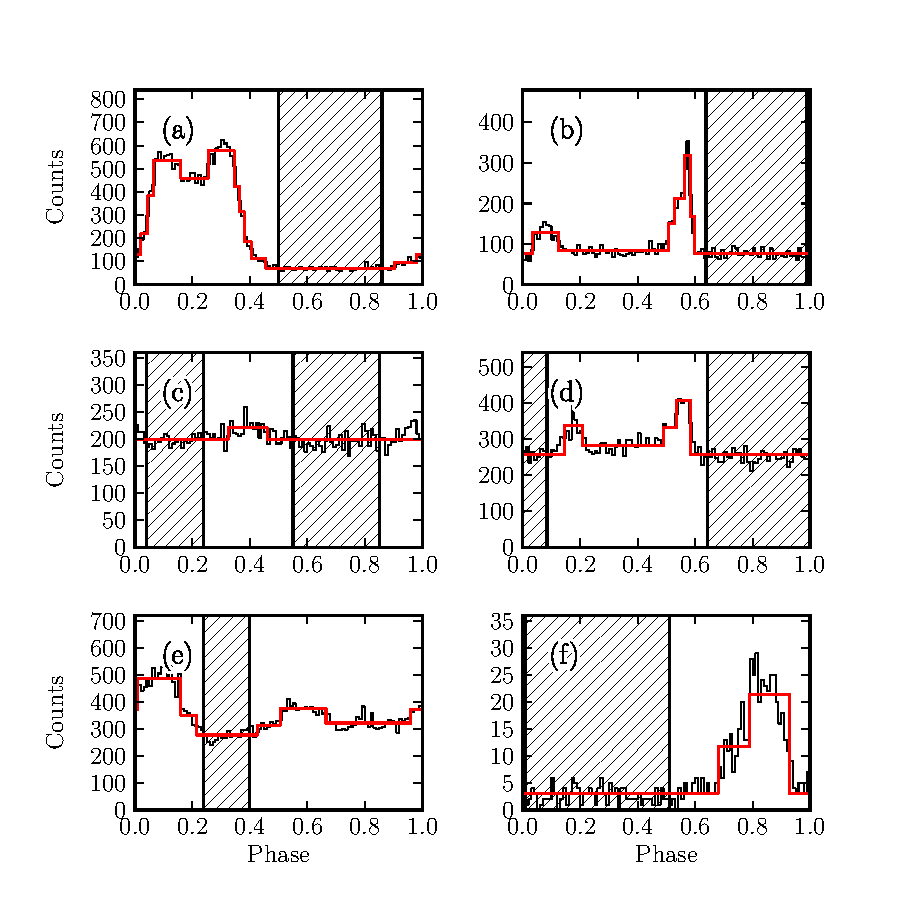
\includegraphics{chapters/offpeak/figures/off_peak_phase_color.pdf}
  \caption{The energy-and-radius optimized light curve, Bayesian block decomposition of the        
  light curve, and off-peak interval for
  (a) PSR J0007+7303, (b) PSR J0205+6449, (c) PSR J1410$-$6132,
  (d) PSR J1747$-$2958, (e) PSR J2021+4026, and (f) PSR J2124$-$3358.
  The black histograms represent the light curves,
  the gray lines (colored red in the electronic version)
  represent the Bayesian block decompositions of the pulsar light curves, and
  the hatched areas represent the off-peak intervals selected by this method.}
  \figlabel{off_peak_select}
\end{figure}


\subsection{Off-peak Analysis Method}
\label{off_peak_analysis}

Characterizing both the spatial and spectral
characteristics of any off-peak emission helps discern its origin.
We employ a somewhat different analysis procedure here than
for the phase-averaged analysis described in Section
\ref{spectralMethodSection}.  To evaluate the spatial characteristics of
any off-peak emission we use the likelihood fitting package \pointlike
\citep[detailed in][]{LAT_collaboration_extended_search_2012}, and
to fit the spectrum we use \gtlike in binned mode via {\it pyLikelihood} as was done for the
phase-averaged analysis.

For each pulsar we start from
the same temporal and spatial event selections described in Section
\ref{obsvSection} but we increase the maximum energy to 400 GeV (the
highest event energy for any ROI under this selection is $\sim$316 GeV).
For the \pointlike analysis we further select a 10$\degree$ radius ROI
and for \gtlike a $14\degree\times14\degree$ square ROI, both centered
on the pulsar postition.  Finally, we only consider photons with 
pulse phases within the corresponding off-peak interval.

We search for off-peak emission
assuming a point source and (except for the Crab Nebula and Vela-X, described below) 
a power-law spectral model.  We fit the position of this
putative off-peak source using \pointlike as described by \citet{2FGL}
and then use the best-fit position in a spectral analysis with \gtlike.
From the spectral analysis we require $TS\geq25$ (just over $4\sigma$)
to claim a detection.  If $TS<25$, we compute upper limits on the flux 
in the energy range from 100 \mev to 316 \gev
assuming
a power law with photon index fixed to 2.0 and a PLEC1 model with
$\Gamma=1.7$ and $E_{\rm cut}=3$ GeV.

The spectrum of the Crab Nebula (associated with PSR J0534+2200) is
uniquely challenging because the GeV spectrum contains both a falling
synchrotron and a rising inverse Compton component \citep{FermiCrab}.
For this particular source we used the best-fit two-component spectral
model from \cite{LAT_collaboration_crab_2012} and fit only the overall
normalization of the source. 
In addition, for Vela-X (associated with PSR J0835-4510) we took the
best-fit spectral model from \cite{FermiVelaX2nd} and fit only the overall
normalization of this source. This spectrum has a smoothly broken power
law spectral model and was fit assuming Vela-X to have an elliptical
disk spatial model.

If the off-peak source is significant, we test whether the spectrum shows
evidence for a cutoff, as described in Section \ref{spectralMethodSection}
and by \citet{LAT_collaboration_PWNCAT_2011}, assuming the source is at
the pulsar position.  We say that the off-peak emission shows evidence for
a cutoff if $TS_{\rm cut}\geq9$, corresponding to a $3\sigma$ detection.

For a significant off-peak point source,
we use \pointlike to test if the emission is significantly
extended.  We assume a radially-symmetric Gaussian source
and fit the position and extension parameter ($\sigma$) as described
in \citet{LAT_collaboration_extended_search_2012}.  The best-fit
extended source parameters are then given to \gtlike, which is used
to fit the spectral parameters and the significance of the extension
over a point source, $TS_{\rm ext}$, evaluated as described in
\citet{LAT_collaboration_extended_search_2012}.  
That paper established that $TS_{\rm ext}\geq16$ means highly probable source extension.
In the present work we aim only to flag possible extension, and use  $TS_{\rm ext}\geq9$.
%% 
%% We say that the off-peak emission shows evidence for extension if $TS_{\rm ext}\geq16$.

To test for variability, even without significant emission over the 3-year time
range, we divide the dataset into 36 intervals and fit the point-source
flux independently in each interval, 
computing $TS_{\rm var}$ as in 2FGL.  
For sources with potential magnetospheric off-peak emission and for
regions with no detection, we performed the test at the pulsar's position.
Otherwise, we test at the best-fit position.
The off-peak emission is said
to show evidence for variability if $TS_{\rm var}\geq91.7$, corresponding
to a $4\sigma$ significance.  
%
As noted in Section \ref{obsvSection}, our timing solutions for PSRs J0205+6449 and J1838$-$0537 are not  
coherent across all three years.  
For these two pulsars, we excluded the time ranges without ephemerides  
and only tested for variability during months that were completely covered.  
For J1838$-$0537 only one month is lost, whereas for J0205+6449 the 7\% data loss is spread across
three separate months.
As a result, $TS_{\rm var}$ for these pulsars is a conservative estimate of variability significance.

The procedure described above, especially the extension analysis,
is particularly sensitive to sources not included in 2FGL that are near the pulsar of interest,
for two reasons.
First, we are using an additional year of data and second,
when ``turning off'' a bright pulsar nearby, faint sources become more
important to the global fit.  Therefore, in many situations we had to run
the analysis several times, iteratively improving the model by including
new sources, until we removed all $TS>25$ residuals. The final
\gtlike-formatted XML source model for each off-peak 
region is included in the auxiliary material.

There are still, however, pulsars for which we were unable to obtain
an unbiased fit of the off-peak emission,
most likely due to inaccuracies in the model of the Galactic diffuse emission
and incorrectly modeled nearby sources.  The most common symptom
of a biased fit is an unphysically large extension.  In these cases,
the extended source attempts to account for multiple point sources or
incorrectly-modeled diffuse emission,
not just the putative off-peak emission.  Systematics associated
with modeling extended sources are discussed more thoroughly in
\citet{LAT_collaboration_extended_search_2012}.  For the purposes of this
catalog, we have flagged the pulsars where off-peak analysis suffered from
these issues and do not attempt a complete understanding of the emission.

Observations of magnetospheric off-peak emission can be used to 
constrain pulsar geometry. Therefore, it is important to know if 
off-peak emission that is otherwise pulsar-like might instead
be incorrectly-modeled Galactic diffuse emission. 
We therefore performed a limited study of the systematics
associated with our model of the Galactic diffuse emission.

For sources which otherwise would be classified as magnetospheric, we
tested the significance of the emission assuming eight different
Galactic diffuse emission models as described in \citet{SNRCatDiffuseSystematics}. 
These models were constructed using a different model building strategy,
vary parameters of the Galactic diffuse emission model, and
have additional degrees of freedom in the fit.

We define $\tsaltdiff$ as the minimum test statistic of any of the
eight alternate diffuse models. This test statistic is computed
assuming the emission to be pointlike at the best-fit position
and is therefore comparable to \tspoint.
For sources which would otherwise be considered magnetospheric,
we flag the emission as potentially 
spurious if $\tsaltdiff<25$.
We caution that although this test can help to 
flag problematic regions,
these models do not probe the entirety of the uncertainty
associated with our model of the Galactic diffuse emission.
Therefore, some diffuse emission could still be incorrectly classified
as magnetospheric.


\subsection{Off-peak Results}
\subseclabel{off_peak_results}

The off-peak intervals of 54 LAT-detected pulsars have
been evaluated by \citet{LAT_collaboration_PWNCAT_2011} using 16 months of sky survey observations.  
This led to the discovery of PWN-like emission
in the off-peak interval of PSR J1023$-$5746, coincident with HESS
J1023$-$575, and identification of 5 pulsars that appear to have near 100\%
duty cycles.  Our results, summarized in Table \ref{tbl-off_peak_table},
extend the analysis to 116 pulsars over 3 years of data.  
Sample off-peak spectra are shown in Figure \ref{off_peak_seds}.
Using the procedures outlined in Sections \ref{peak_definition}
and \ref{off_peak_analysis}, we have identified 34 pulsars that
have significant emission ($TS\geq25$) in their off-peak intervals.
We classify the likely nature of the emission as follows.

If the emission has $TS_{\rm cut}\geq9$, we consider the emission to be
either magnetospheric (`M') or possibly magnetospheric (`M*').
As was discussed in Section \ref{off_peak_analysis}, 
we flag the emission as `M*' if the source is formally spatially extended
($TS_{\rm ext}>16$) or if the source is not robust against varying
the diffuse emission models ($\tsaltdiff<25$). 
On consideration of the angular extent of the PSF of the LAT and inaccuracies in the Galactic diffuse
emission model, we caution against considering the `M*' sources to be definitively classified.
If the source is significantly cutoff, not
significantly extended, and is significant when varying the alternative diffuse models,
we classify the emission as `M'.


On the other hand, if the
emission has $TS_{\rm ext}\geq16$, and does not suffer from confusion as
discussed at the end of Section \ref{off_peak_analysis}, and/or has a hard
photon index, we say it is likely
to originate in the pulsar wind and identify these sources as type `W'.
The remaining sources with off-peak emission not satisfying any of the
previous criteria are identified as type `U' to indicate that the nature
of the emission is unidentified and we do not speculate about its origin.


We identify 9 type `M' sources,
significantly expanding the number of pulsars that perhaps have detectable magnetospheric emission across all rotational phases. 
One caution is that many of these `M' pulsars, especially the young objects, are in regions of particularly bright diffuse gamma-ray
emission, where small fractional uncertainties in the level of diffuse emission can account for much of the apparent unpulsed emission. 
However, if established as true magnetospheric components, these will be important test cases for
pulsar emission models. In addition, we identify ten
`M*'-type regions.
For type `M' and `M*' sources, we present the best-fit spectral parameters using
a point source at the pulsar's position with a PLEC1 spectral model in
%columns 6, 7, and 8 of
Table \ref{tbl-off_peak_table}.  For all other
sources (except the Crab Nebula described in Sec. \ref{off_peak_analysis}), 
we present the spectral results using a power-law spectral
model and the best-fit spatial representation.


Additionally, we identified four off-peak emissions consistent with a PWN
hypothesis, one of them being a new detection at GeV energies (PSR J0205+6449).
Only one of these four, the previously identified Vela$-$X PWN \citep{LAT_collaboration_Vela_X_2010}, is spatially extended for the LAT.
Similarly, we detect six type `U' regions. Three of these are formally 
spatially extended
but because of the spatial systematics 
we assume point-like emission for the spectral analysis.

We mention that for a few sources, the spectral analysis
performed here is in disagreement with the analysis presented in
\citet{LAT_collaboration_PWNCAT_2011}. For soft and faint sources
(including J1044$-$5737 and J1809$-$2332), the spectral discrepancy is
mainly caused by our use of a newer Galactic diffuse model. At lower
energies, small changes in the diffuse model can have a significant
impact on the analysis of a region.  For bright magnetospheric sources
(including J0633+1746 and J2021+4026), the spectral discrepancy is mainly
due to using different phase ranges (see Sec.~\ref{peak_definition}).


\figref{off_peak_luminosity_vs_edot} shows that only
a small fraction of the spindown power goes into 
the gamma-ray emission from LAT-detected PWNe.
Similarly, 
Figure~\ref{P0_sqEDOTD2} shows that the LAT only detects
PWNe from the youngest pulsars with the highest spindown power.
GeV emission from the Crab Nebula is highly time variable (Section \ref{off_peak_analysis}).  
Indeed, we find
$TS_{\rm var}=373$ for the Crab Nebula; however
no other source demonstrated flux variability (all have $16 <TS_{\rm var} <65)$.  
Other GeV PWNe may be variable, but the combination of lower fluxes
and less-extreme variations limits our ability identify them as such.


The off-peak results for several interesting sources are
presented in Appendix~\ref{App-off_peak_individual_source_discussion}.
The complete off-peak search results can be found in the accompanying
auxiliary information described in Appendix \ref{off_peak_auxiliary}.
For regions where we find $TS<25$, the auxiliary information contains
upper limits computed for both a power-law spectral model and a
PLEC1 model with $E_{\rm cut}=3$ GeV and $\Gamma=1.7$.  The auxiliary
information also contains $TS_{\rm var}$ for each off-peak interval.



\begin{deluxetable}{ll*{8}c}
\tablecolumns{8}
\tablewidth{0pt}
\tabletypesize{\scriptsize}
\tablecaption{Off-Peak Spatial and Spectral Results
\label{tbl-off_peak_table}
}
\tablehead{\colhead{PSR} & \colhead{Type} & \colhead{$\tspoint$} & \colhead{$\tsext$} & \colhead{$\tscutoff$} & \colhead{$\tsaltdiff$} & \colhead{Energy Flux} & \colhead{$\Gamma$} & \colhead{$\Ecutoff$}\\ \colhead{ } & \colhead{ } & \colhead{ } & \colhead{ } & \colhead{ } & \colhead{ } & \colhead{($10^{-11}\,\efluxunits$)} & \colhead{ } & \colhead{(GeV)}}
\startdata
\multicolumn{8}{c}{Young Pulsars} \\[3pt]
\hline
J0007+7303 & U & 71.4 & 10.8 & 0.0 &  & $1.98 \pm 0.26$ & $2.61 \pm 0.14$ &  \\
J0205+6449 & W & 33.7 & 0.5 & 0.0 &  & $1.75 \pm 0.68$ & $1.61 \pm 0.21$ &  \\
J0534+2200 & W & 5247. & 0.0 & 0.3 &  & $67.2 \pm 1.6$ & \tablenotemark{a} &  \\
J0631+1036 & U & 33.1 & 0.0 & 5.4 &  & $1.70 \pm 0.33$ & $2.38 \pm 0.14$ &  \\
J0633+1746 & M & 3666. & 2.3 & 239. & 3369. & $41.4 \pm 1.1$ & $1.37 \pm 0.09$ & $0.93 \pm 0.10$ \\
J0734$-$1559 & M* & 28.3 & 12.4 & 30.8 & 0.0 & $1.61 \pm 0.24$ & $0.01 \pm 0.08$ & $0.17 \pm 0.03$ \\
J0835$-$4510 & W & 473. & 283. & 22.8 &  & $30.3 \pm 1.2$ & \tablenotemark{b} &  \\
J0908$-$4913 & M* & 65.1 & 41.4 & 60.4 & 3.1 & $3.04 \pm 1.07$ & $0.15 \pm 0.59$ & $0.30 \pm 0.01$ \\
J1023$-$5746 & M* & 59.7 & 30.0 & 10.9 & 72.5 & $5.35 \pm 1.17$ & $0.57 \pm 0.80$ & $0.49 \pm 0.21$ \\
J1044$-$5737 & M* & 42.0 & 98.1 & 22.4 & 25.6 & $3.12 \pm 0.75$ & $0.80 \pm 0.93$ & $0.40 \pm 0.18$ \\
J1105$-$6107 & M* & 33.3 & 37.5 & 21.7 & 39.4 & $3.81 \pm 0.77$ & $0.92 \pm 0.56$ & $0.48 \pm 0.22$ \\
J1112$-$6103 & U & 65.0 & 71.1 & 0.9 &  & $5.10 \pm 0.74$ & $2.17 \pm 0.09$ &  \\
J1119$-$6127 & U & 61.3 & 1.0 & 0.9 &  & $4.11 \pm 0.63$ & $2.22 \pm 0.09$ &  \\
J1124$-$5916 & M & 95.9 & 0.0 & 18.2 & 59.4 & $2.87 \pm 0.71$ & $1.31 \pm 0.91$ & $1.43 \pm 1.42$ \\
J1410$-$6132 & U & 27.5 & 71.2 & 0.4 &  & $4.29 \pm 1.05$ & $1.90 \pm 0.15$ &  \\
J1513$-$5908 & W & 102. & 3.5 & 0.0 &  & $4.95 \pm 0.83$ & $1.78 \pm 0.12$ &  \\
J1620$-$4927 & M* & 28.9 & 0.5 & 35.2 & 0.0 & $5.25 \pm 0.96$ & $0.35 \pm 0.94$ & $0.57 \pm 0.29$ \\
J1746$-$3239 & M* & 53.3 & 34.3 & 34.2 & 0.0 & $3.65 \pm 0.59$ & $0.94 \pm 0.31$ & $0.60 \pm 0.10$ \\
J1747$-$2958 & M & 45.5 & 5.4 & 49.8 & 50.4 & $8.41 \pm 2.84$ & $0.02 \pm 0.32$ & $0.28 \pm 0.01$ \\
J1809$-$2332 & M* & 32.5 & 13.6 & 21.9 & 0.0 & $4.10 \pm 0.80$ & $0.24 \pm 0.83$ & $0.31 \pm 0.11$ \\
J1813$-$1246 & M & 62.8 & 0.0 & 9.0 & 49.7 & $6.31 \pm 1.40$ & $1.60 \pm 0.73$ & $0.99 \pm 0.95$ \\
J1836+5925 & M & 10407. & 0.0 & 365. & 10401. & $36.9 \pm 0.7$ & $1.47 \pm 0.03$ & $1.98 \pm 0.09$ \\
J1838$-$0537 & M* & 51.3 & 32.9 & 21.9 & 41.9 & $8.35 \pm 1.31$ & $1.39 \pm 0.54$ & $2.55 \pm 2.48$ \\
J2021+4026 & M & 1717. & 8.7 & 244. & 1978. & $64.0 \pm 1.4$ & $1.64 \pm 0.02$ & $1.82 \pm 0.04$ \\
J2032+4127 & U & 53.6 & 76.1 & 1.5 &  & $4.36 \pm 0.77$ & $2.07 \pm 0.12$ &  \\
J2055+2539 & M & 123. & 0.0 & 30.0 & 101. & $1.63 \pm 0.19$ & $1.05 \pm 0.28$ & $0.64 \pm 0.12$ \\
\hline\\[-5pt]
\multicolumn{8}{c}{Millisecond Pulsars} \\[3pt]
\hline
J0034$-$0534 & U & 41.0 & 0.0 & 6.0 &  & $0.82 \pm 0.16$ & $2.40 \pm 0.19$ &  \\
J0102+4839 & U & 49.7 & 0.0 & 7.4 &  & $1.29 \pm 0.20$ & $2.51 \pm 0.14$ &  \\
J0218+4232 & U & 50.1 & 0.0 & 6.8 &  & $2.13 \pm 0.33$ & $2.72 \pm 0.26$ &  \\
J0340+4130 & M* & 26.9 & 0.1 & 16.3 & 11.9 & $0.53 \pm 0.11$ & $0.02 \pm 0.22$ & $0.94 \pm 0.28$ \\
J1658$-$5324 & U & 42.3 & 0.0 & 1.9 &  & $1.69 \pm 0.29$ & $2.52 \pm 0.76$ &  \\
J2043+1711 & U & 52.5 & 0.0 & 8.8 &  & $1.46 \pm 0.27$ & $2.29 \pm 0.14$ &  \\
J2124$-$3358 & M & 129. & 0.0 & 19.8 & 118. & $1.08 \pm 0.15$ & $0.70 \pm 0.51$ & $1.21 \pm 0.49$ \\
J2302+4442 & M & 114. & 0.0 & 9.8 & 105. & $1.45 \pm 0.20$ & $1.54 \pm 0.40$ & $1.61 \pm 0.82$ \\
\enddata


\tablenotetext{a}{The spectral shape of the Crab Nebula was taken from \citet{LAT_collaboration_crab_2012}.}
\tablenotetext{b}{The spectral shape of Vela$-$X was taken from \cite{FermiVelaX2nd}.}

\tablecomments{Off-peak regions with a significant detection of emission.
The source classification is `M' for likely magnetospheric, 
`M*' for possibly magnetospheric but with a problematic spatial analysis or in a region with possibly poorly-modeled
Galactic diffuse emission,
`W' for likely pulsar wind, and `U' for unidentified.
The table includes the significance of the source ($TS$),  
of the source extension ($TS_{\rm ext}$), of a spectral cutoff ($TS_{\rm cut}$),
and with the alternative diffuse models ($\tsaltdiff$). 
The best-fit energy flux and photon index are computed in the energy range from 100 \mev to 316 \gev.
For sources with large $TS_{\rm cut}$, the exponential cutoff energies are presented. 
The quoted errors are statistical only. A few sources are discussed in Section~\ref{off_peak_individual_source_discussion}.
}


\end{deluxetable}

\begin{figure}
  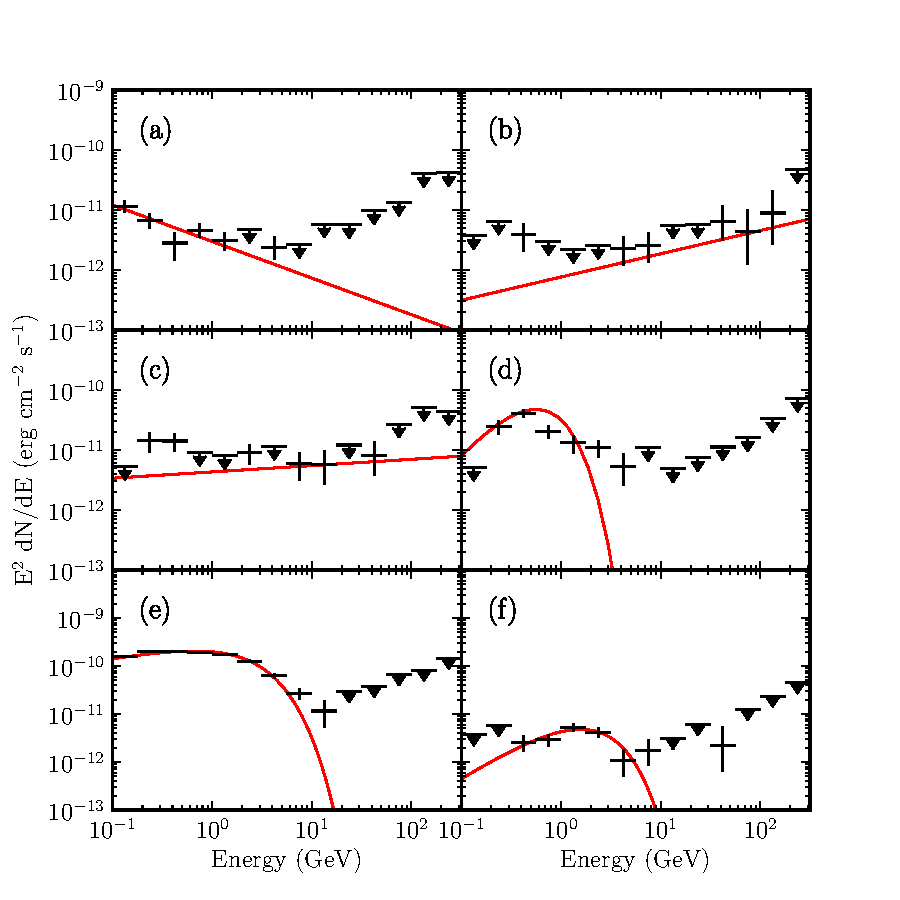
\includegraphics{chapters/offpeak/figures/off_peak_seds_color.pdf}
  \caption{Spectral energy distributions for the off-peak
  phase intervals around
  (a) PSR J0007+7303 (b) PSR J0205+6449, (c) PSR J1410$-$6132,
  (d) PSR J1747$-$2958, (e) PSR J2021+4026, and (f) PSR J2124$-$3358.
  We plot a detection in those energy bands in which the source is found with $TS\geq4$ (a $2\sigma$ detection) and report a Bayesian 95\% confidence-level upper limit otherwise.  The best-fit spectral model, using the full energy range, is also shown for comparison.
  }
  \label{off_peak_seds}
\end{figure}

\begin{figure}
  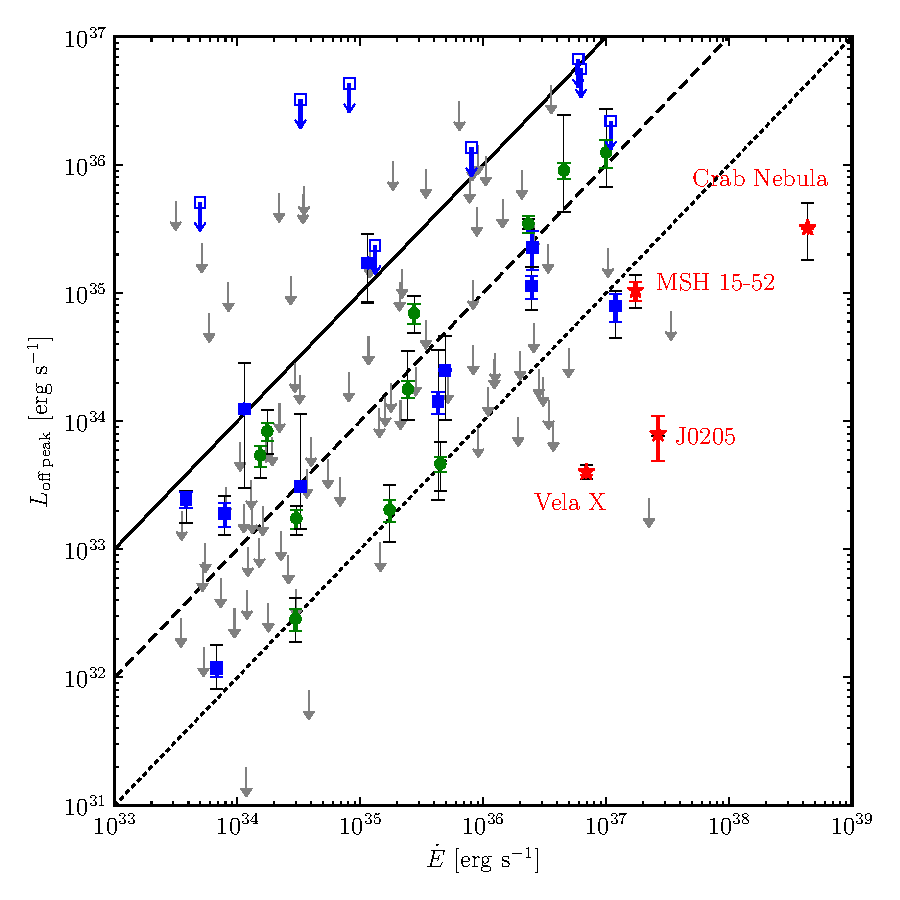
\includegraphics{chapters/offpeak/figures/off_peak_luminosity_vs_edot_color.pdf}
  \caption{The off-peak luminosity compared to the observed pulsar spindown power. 
  The luminosity is computed and plotted with the same convention as
  Figure~\ref{EDotLumG}. A luminosity upper limit is plotted
  when there is no significant off-peak emission or when there
  is only a distance upper limit.
  The
  star-shaped markers (colored red in the online version) represent
  type `W' sources, the square-shaped markers (colored blue) represent type `M' 
  and `M*' sources, 
  circular markers (colored green) represent type `U' sources,
  and the gray arrows represent non-detections.
  The filled blue square-shaped markers represent `M' and `M*' sources
  with a detected luminosity and the unfilled markers represent luminosity
  upper limits where there is only a distance upper limit.
  The solid, dashed, and dotted diagonals show 100\%, 10\%, and 1\% efficiency
  (respectively).
  }
  \figlabel{off_peak_luminosity_vs_edot}
\end{figure}

\section{Off-Peak Individual Source Discussion}
\label{off_peak_individual_source_discussion}

Here we discuss several interesting sources found in the off-peak
analysis presented in Section~\ref{unpulsed}.

% J0007+7303
The off-peak emission from PSR J0007+7303 in the SNR CTA1 was previously studied by \cite{Fermi_CTA1_2012}.
They found a soft and not-significantly cut off source in the off-peak region that
is marginally extended.
We find a similar spectrum and extension significance ($TS_{\rm ext}=10.8$), and therefore classify this
source as type `U'.


% J0205+6449
The new type `W' source is associated with PSR J0205+6449 \citep{LATPSR0205}.
The off-peak spectrum for this source is shown in panel b of Figure
\ref{off_peak_seds}.  The emission is best fit as a point source at
$(l,b)=(130\fdg73,3\fdg11)$ with a 95\% confidence-level radius of $0\fdg03$.
The source has a hard spectrum (power law with $\Gamma=1.61\pm0.21$)
and is therefore consistent with a PWN hypothesis.
This nebula has been observed at infrared
\citep{3C58_IR_PWN} and X-ray \citep{3C58_Xray_PWN} energies. This
suggests that we could be observing the inverse Compton emission from
the same electrons powering synchrotron emission at lower energies.
The PWN hypothesis is supported by the associated pulsar's
very high $\dot E=2.6\times10^{36}$ erg s$^{-1}$ and relatively young
characteristic age, $\tau_c = 5400$ yr. This is consistent with the properties
of other pulsars with LAT-detected PWN, and we favor a PWN
interpretation.
We note that the discrepancy between our spectrum and the upper limit
quoted in \citet{LAT_collaboration_PWNCAT_2011} is mainly caused by
our expanded energy range and because the flux upper limit was computed
assuming a different spectral index.


However, we note that PSR J0205+6449 is associated to the SNR 3C58
(G130.7+3.1).  Given the 2 kpc distance estimate from Section \ref{Distances}
and the density of thermal material estimated by \cite{3C58_Xray_PWN}, we can estimate
the energetics required for the LAT emission to originate in the SNR.
Following the prescription in \cite{Gamma_Visibility_SNRs_Drury_1994},
we assume the LAT emission to be hadronic and estimate a cosmic-ray
efficiency for the SNR of $\sim10$\%, which is energetically allowed.
We therefore cannot rule out the SNR hypothesis.

No TeV detection of this source has been reported, but given the hard photon
index at GeV energies this is a good candidate for observations by
an atmospheric Cherenkov telescope. Improved spectral and spatial observations 
at TeV energies might help to uniquely classify the emission.

We obtain a flux for Vela-X which is $\sim10\%$ larger than the flux
obtained in \cite{FermiVelaX2nd}. This discrepancy is most-likey due to
assuming a different spatial model for the emission (radially-symmetric
Gaussian compared to elliptical Gaussian).

% J1023-575
PSR J1023$-$5746 is associated with the TeV PWN HESS J1023$-$575
\citep{HESS_J1023-575_HESS_Collaboration_2007}.  LAT emission from
this PWN was first reported in \citet{LAT_collaboration_PWNCAT_2011}.
Because of the dominant low-energy magnetospheric emission, we classify
this as type `M' and not as a PWN.
A phase-averaged analysis of this source for energies above 10 GeV is
reported in \citet{Rousseau2013}. 


% J1119-6127
PSR J1119$-$6127 \citep{FermiMagnetars} is associated with the TeV source HESS
J1119$-$614\footnote{The discovery of HESS J1119$-$614 was presented at the
``Supernova Remnants and Pulsar Wind Nebulae in the Chandra Era'' in
2009. See \url{http://cxc.harvard.edu/cdo/snr09/pres/DjannatiAtai\_Arache\_
v2.pdf}.}. Our off-peak analysis 
classifies this source as `U' because its spectrum is soft and not significantly
cut off. However, the SED appears to represent a cutoff spectrum at low
energy and a hard rising spectrum at high energy.  
\citet{Rousseau2013} significantly detect this PWN using the analysis procedure as described for J1023$-$575.
We are likely detecting a composite of magnetospheric emission at low energy and pulsar-wind emission
at high energy.


% J1357-6429
PSR J1357$-$6429 \citep{LAT_J1357} has an associated PWN HESS J1356$-$645 detected at
TeV energies \citep{HESS_HESS_J1356-645_2011}.  Our analysis of the off-peak regions surrounding PSR
J1357$-$6429 shows a source positionally and spectrally consistent with
HESS J1356$-$645, but with significance just below detection threshold ($TS=21.0$).  
\citet{Rousseau2013} present significant emission from this source.

% J1410-6132
The off-peak region of PSR J1410$-$6132 \citep{OBrien_2008} shows a relatively hard
spectral index of $1.90\pm0.15$, and the spectrum is not significantly
cut off.  There is no associated TeV PWN
and enough low-energy GeV emission is present to caution against a clear
PWN interpretation.  We classify this source as `U', but
further observations could reveal interesting emission.

% J2021+4026
PSR J2021+4026 is spatially coincident with the
LAT-detected and spatially extended Gamma Cygni SNR
\citep{LAT_collaboration_extended_search_2012}.  The off-peak emission
from this pulsar is consistent with an exponentially-cutoff spectrum and
is therefore classified as type `M'.  The source's marginal extension
($TS_{\rm ext}=8.7$) is likely due to some contamination from the SNR.





\chapter{Search for \acp{PWN} associated with TeV Pulsars}

\section{List of Candidates}

\section{Analysis Method}

\section{Sources Detected}


\chapter{Search for \acp{PWN} associated with High Edot Pulsars}

\chapter{Population Study of LAT-detected \acp{PWN}}

% and the end material

\appendix

%\include{appendix1}
%\include{appendix2}
%\include{appendix3}


% bibliography style came from 
%  http://ads.harvard.edu/pubs/bibtex/astronat/apj/apj.bst
\bibliographystyle{macros/apj}

\bibliography{lande_thesis_stanford}

\end{document}

